\subsection{Evolución de la web}

La evolución de los servicios proporcionados a través de internet ha sido drástica puesto que ha cambiado el modo de vida de las personas. En la figura \ref{fig:utilizacion_internet} se evidencia que el crecimiento de internet (de los servicios que en ella se soportan) se da en función de los servicios de conectividad social que son creados y soportados en ella. La web 1.0 fue utilizada en mayor medida por científicos para el intercambio de información en formato hipertexto. No había una interacción fuerte entre cada científico sino que ellos acudían a internet para buscar o poner a disposición material científico. Con la venida de la web 2.0 y la introducción de la interacción del usuario con la web, generando contenido en tiempo real, fueron creados servicios de redes sociales en-línea (OSN en inglés: On-line Social Network), produciendo una partición en los tipos de redes sociales. Así, las redes sociales a las que pertenece el ser humano en la era digital se dividieron convenientemente en “redes sociales fuera de línea” y “redes sociales en línea” (Offline Social Network y Online Social Network) \cite{dynamics}.

\begin{figure}[!htb]
  \begin{center}
    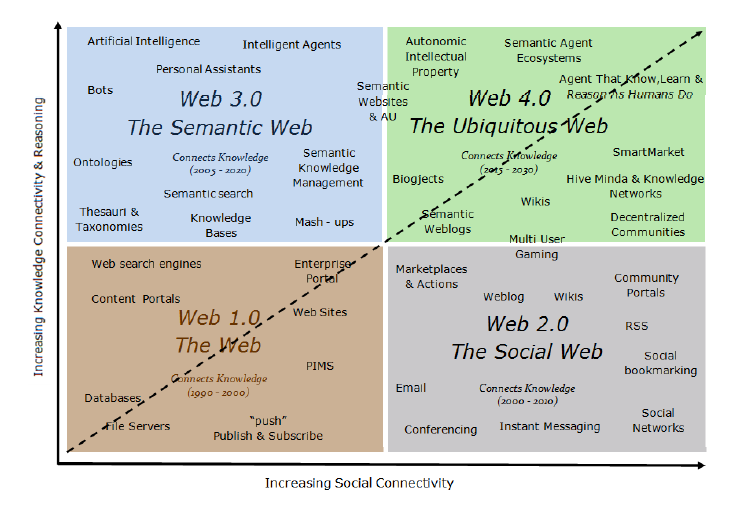
\includegraphics[width=11cm]{./imagenes/utilizacion_internet.png}
    \caption{Cambio de la utilización de internet en función de los servicios de conectividad social que son creados y soportados en ella}
    \label{fig:utilizacion_internet}
    \textbf{Fuente:}  http://goo.gl/3jGPPJ - Evolución de la web. Lozada, Pablo.
  \end{center}
\end{figure}
